\documentclass[11pt,a4paper]{article}
\usepackage[margin=2.3cm]{geometry}
\usepackage[T1]{fontenc}
\usepackage{textcomp}
\input{glyphtounicode}
\pdfgentounicode=1
\usepackage{lmodern}
\usepackage{amsmath}
\usepackage{xcolor}
\usepackage{listings}
\usepackage{tcolorbox}
\tcbuselibrary{breakable}
\usepackage{booktabs}
\usepackage{array}
\usepackage{tikz}
\usepackage{float}
\usepackage{graphicx}
\graphicspath{{images/}}
\usepackage{hyperref}
\hypersetup{colorlinks=true, linkcolor=blue!50!black, citecolor=green!40!black}

\usepackage{accsupp}
% line numbers are drawn but excluded from copied text
\newcommand{\nocopy}[1]{\BeginAccSupp{method=escape,ActualText={}}#1\EndAccSupp{}}
\lstset{
  language=C, basicstyle=\ttfamily\small, keywordstyle={}, commentstyle={}, stringstyle={},
  numbers=left, numberstyle=\footnotesize\nocopy, numbersep=10pt, xleftmargin=2.4em,
  frame=none, columns=fullflexible, keepspaces=true, upquote=true, showstringspaces=false,
  breaklines=true, captionpos=b, aboveskip=1em, belowskip=0.8em
}
\lstdefinestyle{sh}{language=bash, numbers=none, xleftmargin=2.4em}
\renewcommand{\lstlistingname}{Listing}
% code names in the text: grey monospace
\let\origtexttt\texttt
\renewcommand{\texttt}[1]{\textcolor{black!60}{\origtexttt{#1}}}

\newcommand{\cbx}[2]{\colorbox{#1}{\makebox[0.65em]{\strut #2}}}
\newcommand{\sm}[1]{\cbx{green!22}{#1}}
\newcommand{\pv}[1]{\cbx{orange!35}{#1}}
\newcommand{\cd}[1]{\cbx{violet!15}{#1}}
\newcommand{\nn}[1]{\cbx{white}{#1}}
% value that changed since the previous step
\newcommand{\chg}[1]{\textcolor{red!80!black}{\textbf{#1}}}
\tikzset{cell/.style={draw=gray!60, minimum width=0.75cm, minimum height=0.75cm, font=\small},
  cn/.style={cell, fill=white}, cb/.style={cell, fill=blue!22}, ct/.style={cell, fill=teal!28},
  cp/.style={cell, fill=orange!35, very thick}, cs/.style={cell, fill=green!22}, cv/.style={cell, fill=violet!15}}
% \arr{v/style,...}: one row of 8 cells with indices above
\newcommand{\arr}[1]{%
  \foreach \v/\c [count=\k from 0] in {#1} {
    \node[\c] at (0.85*\k,0) {\v};
    \node[font=\tiny, text=gray] at (0.85*\k,0.6) {\k};
  }}
\newtcolorbox{keyidea}{colback=blue!4, colframe=blue!45!black, title=Key ideas, fonttitle=\bfseries\small}
\newtcolorbox{experiment}{breakable, colback=orange!5, colframe=orange!70!black, title=Experiment, fonttitle=\bfseries\small}

\title{\textbf{OpenMP Tasks: Parallel Quicksort}\\[4pt]\large Lesson 12, second example: \texttt{task} on a recursive, irregular algorithm}
\author{Gustavo Lozano}
\date{November 2026}

\begin{document}
\maketitle

\noindent\textit{\small Source: van der Pas, Stotzer \& Terboven~\cite{vdp}, chapter on
tasking. Prerequisite: \texttt{openmp\_tasks.pdf} (Lesson 12).}

\section{Why this example}
Fibonacci showed the mechanics of tasks, but its call tree is regular: the work could be
predicted in advance. Quicksort is the opposite. Each step picks a pivot, moves the smaller
values to the left and the larger ones to the right (the \emph{partition}), and then sorts
both sides. How big each side is depends on the data and is only known after the
partition:
\begin{itemize}
  \item the work is a \textbf{tree}, not a loop: \texttt{omp for} cannot express it;
  \item the pieces have \textbf{unpredictable sizes}: no static split can balance them.
\end{itemize}

\begin{figure}[H]
\centering
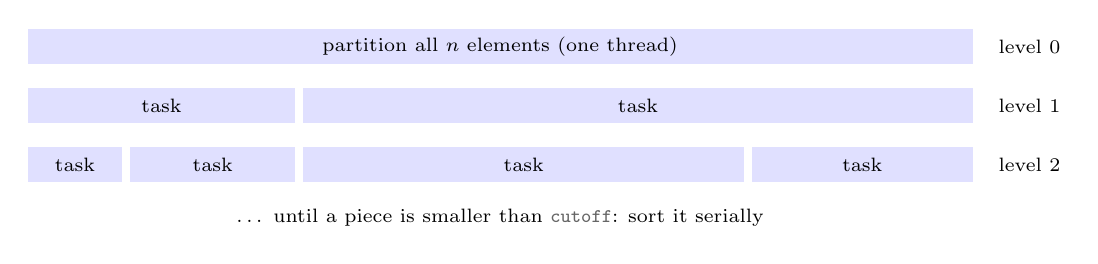
\begin{tikzpicture}[thick, x=1cm, y=0.75cm]
  \fill[blue!12] (0,0) rectangle (12,0.6); \node[font=\scriptsize] at (6,0.3) {partition all $n$ elements (one thread)};
  \fill[blue!12] (0,-1) rectangle (3.4,-0.4); \fill[blue!12] (3.5,-1) rectangle (12,-0.4);
  \node[font=\scriptsize] at (1.7,-0.7) {task}; \node[font=\scriptsize] at (7.75,-0.7) {task};
  \fill[blue!12] (0,-2) rectangle (1.2,-1.4); \fill[blue!12] (1.3,-2) rectangle (3.4,-1.4);
  \fill[blue!12] (3.5,-2) rectangle (9.1,-1.4); \fill[blue!12] (9.2,-2) rectangle (12,-1.4);
  \node[font=\scriptsize] at (0.6,-1.7) {task}; \node[font=\scriptsize] at (2.35,-1.7) {task};
  \node[font=\scriptsize] at (6.3,-1.7) {task}; \node[font=\scriptsize] at (10.6,-1.7) {task};
  \node[font=\scriptsize, anchor=west] at (12.2,0.3) {level 0};
  \node[font=\scriptsize, anchor=west] at (12.2,-0.7) {level 1};
  \node[font=\scriptsize, anchor=west] at (12.2,-1.7) {level 2};
  \node[font=\scriptsize] at (6,-2.6) {\ldots\ until a piece is smaller than \texttt{cutoff}: sort it serially};
\end{tikzpicture}
\caption{Each partition splits its range in two pieces of unpredictable size; each piece
becomes a task.}
\end{figure}

\paragraph{Intuition: who does what, and when.} Figure~2 follows an example with $n=100$
elements and \texttt{cutoff} $=40$, run by 2 threads. To keep the numbers simple, assume a
partition of $m$ elements costs $m$ time units and a serial sort of $m$ elements costs $3m$.

\begin{figure}[H]
\centering
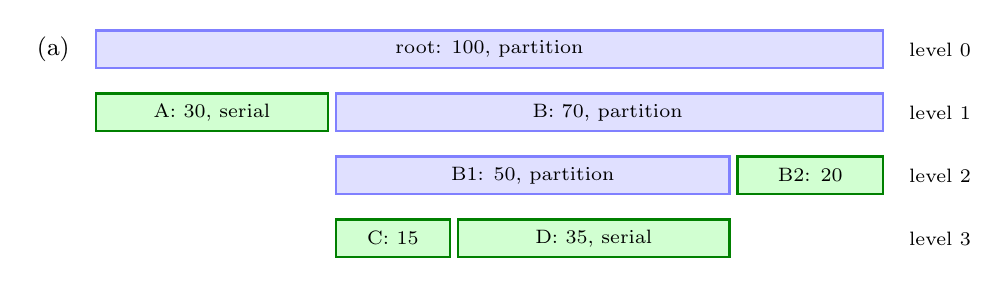
\begin{tikzpicture}[thick, x=0.1cm, y=0.8cm, font=\scriptsize,
  pt/.style={draw=blue!50, fill=blue!12}, sr/.style={draw=green!50!black, fill=green!18}]
  
  \node[anchor=east, font=\small] at (-2,0.8) {(a)};
  \draw[pt] (0,0.5) rectangle (100,1.1);   \node at (50,0.8) {root: 100, partition};
  \draw[sr] (0,-0.5) rectangle (29.5,0.1); \node at (14.75,-0.2) {A: 30, serial};
  \draw[pt] (30.5,-0.5) rectangle (100,0.1); \node at (65,-0.2) {B: 70, partition};
  \draw[pt] (30.5,-1.5) rectangle (80.5,-0.9); \node at (55.5,-1.2) {B1: 50, partition};
  \draw[sr] (81.5,-1.5) rectangle (100,-0.9); \node at (90.75,-1.2) {B2: 20};
  \draw[sr] (30.5,-2.5) rectangle (45,-1.9); \node at (37.75,-2.2) {C: 15};
  \draw[sr] (46,-2.5) rectangle (80.5,-1.9); \node at (63.25,-2.2) {D: 35, serial};
  \node[anchor=west] at (102,0.8) {level 0};
  \node[anchor=west] at (102,-0.2) {level 1};
  \node[anchor=west] at (102,-1.2) {level 2};
  \node[anchor=west] at (102,-2.2) {level 3};
\end{tikzpicture}

\vspace{4mm}
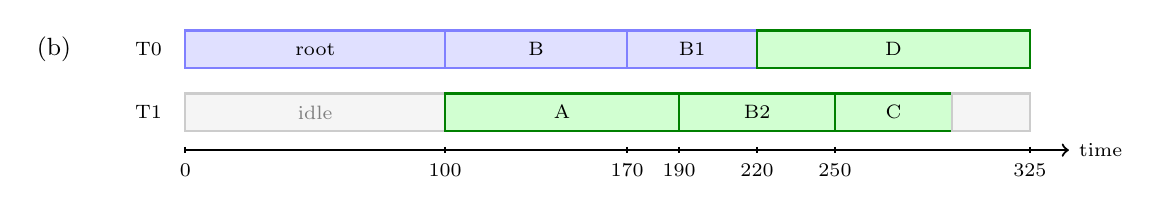
\begin{tikzpicture}[thick, x=0.033cm, y=0.8cm, font=\scriptsize,
  pt/.style={draw=blue!50, fill=blue!12}, sr/.style={draw=green!50!black, fill=green!18},
  idl/.style={draw=gray!40, fill=gray!8}]
  \node[anchor=east, font=\small] at (-40,0.3) {(b)};
  \node[anchor=east] at (-5,0.3) {T0}; \node[anchor=east] at (-5,-0.7) {T1};
  
  \draw[pt] (0,0) rectangle (100,0.6);   \node at (50,0.3) {root};
  \draw[pt] (100,0) rectangle (170,0.6); \node at (135,0.3) {B};
  \draw[pt] (170,0) rectangle (220,0.6); \node at (195,0.3) {B1};
  \draw[sr] (220,0) rectangle (325,0.6); \node at (272.5,0.3) {D};
  
  \draw[idl] (0,-1) rectangle (100,-0.4);  \node[text=gray] at (50,-0.7) {idle};
  \draw[sr] (100,-1) rectangle (190,-0.4); \node at (145,-0.7) {A};
  \draw[sr] (190,-1) rectangle (250,-0.4); \node at (220,-0.7) {B2};
  \draw[sr] (250,-1) rectangle (295,-0.4); \node at (272.5,-0.7) {C};
  \draw[idl] (295,-1) rectangle (325,-0.4);
  
  \draw[->] (0,-1.3) -- (340,-1.3) node[right] {time};
  \foreach \t in {0,100,170,190,220,250,325} {
    \draw (\t,-1.25) -- (\t,-1.35); \node[below] at (\t,-1.35) {\t};
  }
\end{tikzpicture}
\caption{(a) Tasks and their sizes; blue: partition and create two tasks, green: below the
cutoff, sorted serially. (b) A possible timeline with 2 threads: a thread that becomes free
takes the next task in the queue.}
\end{figure}

\noindent What Figure~2 shows:
\begin{itemize}
  \item The sizes 30/70, then 50/20, then 15/35 are only known after each partition; nobody
        could have assigned the work in advance.
  \item No thread is told what to do: T1 takes A because it is free at time 100; it takes B2
        at 190 and C at 250 for the same reason.
  \item The run takes 325 time units instead of $520$ serially ($100+70+50$ for partitions,
        $3\cdot(30+20+15+35)$ for serial sorts): a speed-up of 1.6 with 2 threads.
  \item T1 is idle at the start, because only one piece exists until the first partition ends,
        and at the end, because D is the largest last task. These two effects limit the
        speed-up (see the experiment).
\end{itemize}

\section{Quicksort by hand (one thread)}
The array to sort, with its indices above each element ($n = 8$):
\begin{center}
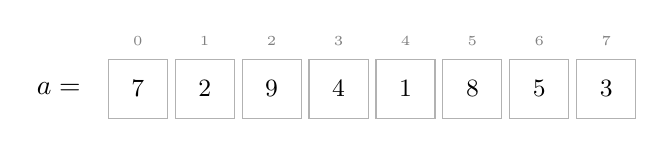
\begin{tikzpicture}
  \node[anchor=east] at (-0.6,0) {$a =$};
  \arr{7/cn,2/cn,9/cn,4/cn,1/cn,8/cn,5/cn,3/cn}
\end{tikzpicture}
\end{center}
We follow the call (Listing~\ref{lst:qs}), with \texttt{OMP\_NUM\_THREADS=1}:
\[
  \texttt{quicksort\_tasks(a,\ lo = 0,\ hi = 7,\ cutoff = 3)}
\]
With one thread, tasks wait in a queue and T0 runs them in creation order.

\begin{center}
\small
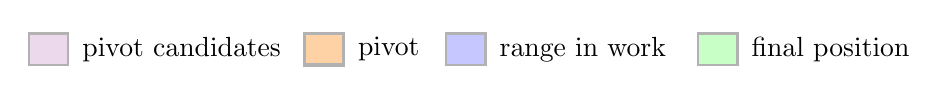
\begin{tikzpicture}[thick]
  \node[cv, minimum width=0.5cm, minimum height=0.4cm] at (0,0) {};   \node[right] at (0.3,0) {pivot candidates};
  \node[cp, minimum width=0.5cm, minimum height=0.4cm] at (3.5,0) {};  \node[right] at (3.8,0) {pivot};
  \node[cb, minimum width=0.5cm, minimum height=0.4cm] at (5.3,0) {};  \node[right] at (5.6,0) {range in work};
  \node[cs, minimum width=0.5cm, minimum height=0.4cm] at (8.5,0) {};  \node[right] at (8.8,0) {final position};
\end{tikzpicture}
\end{center}

%-------------------------------------------------------------------
\subsection*{Stage 1 \quad call \texttt{(0,7)}: \texttt{hi-lo} $= 7 \ge$ \texttt{cutoff} $= 3$ $\Rightarrow$ partition and create two tasks}

\paragraph{1a. Pivot: median of three.} $\texttt{mid} = 0 + (7-0)/2 = 3$.
\begin{center}
\small
\begin{tabular}{@{}lll@{}}
\toprule
Test & Action & $a[0], \dots, a[7]$ \\ \midrule
start & --- & \cd{7} \nn{2} \nn{9} \cd{4} \nn{1} \nn{8} \nn{5} \cd{3} \\
$a[3]=4 < a[0]=7$ & \texttt{swap(a, 3, 0)} & \cd{\chg{4}} \nn{2} \nn{9} \cd{\chg{7}} \nn{1} \nn{8} \nn{5} \cd{3} \\
$a[7]=3 < a[0]=4$ & \texttt{swap(a, 7, 0)} & \cd{\chg{3}} \nn{2} \nn{9} \cd{7} \nn{1} \nn{8} \nn{5} \cd{\chg{4}} \\
$a[7]=4 < a[3]=7$ & \texttt{swap(a, 7, 3)} & \cd{3} \nn{2} \nn{9} \cd{\chg{4}} \nn{1} \nn{8} \nn{5} \cd{\chg{7}} \\
$3 \le 4 \le 7$ & \texttt{swap(a, 3, 7)}: median to the end & \nn{3} \nn{2} \nn{9} \nn{\chg{7}} \nn{1} \nn{8} \nn{5} \pv{\chg{4}} \\
\bottomrule
\end{tabular}
\end{center}

\paragraph{1b. Scan with pivot $=4$.} \texttt{i} = next slot for a value $<$ pivot;
\texttt{j} visits $a[0..6]$. Green: values already known to be $<$ pivot.
\begin{center}
\small
\begin{tabular}{@{}cccll@{}}
\toprule
\texttt{j} & \texttt{i} & $a[j] <$ pivot & Action & $a[0], \dots, a[7]$ \\ \midrule
0 & 0 & true & \texttt{swap(a, 0, 0)} & \sm{3} \nn{2} \nn{9} \nn{7} \nn{1} \nn{8} \nn{5} \pv{4} \\
1 & 1 & true & \texttt{swap(a, 1, 1)} & \sm{3} \sm{2} \nn{9} \nn{7} \nn{1} \nn{8} \nn{5} \pv{4} \\
2 & 2 & false & --- & \sm{3} \sm{2} \nn{9} \nn{7} \nn{1} \nn{8} \nn{5} \pv{4} \\
3 & 2 & false & --- & \sm{3} \sm{2} \nn{9} \nn{7} \nn{1} \nn{8} \nn{5} \pv{4} \\
4 & 2 & true & \texttt{swap(a, 2, 4)} & \sm{3} \sm{2} \sm{\chg{1}} \nn{7} \nn{\chg{9}} \nn{8} \nn{5} \pv{4} \\
5 & 3 & false & --- & \sm{3} \sm{2} \sm{1} \nn{7} \nn{9} \nn{8} \nn{5} \pv{4} \\
6 & 3 & false & --- & \sm{3} \sm{2} \sm{1} \nn{7} \nn{9} \nn{8} \nn{5} \pv{4} \\
\bottomrule
\end{tabular}
\end{center}

\paragraph{1c. Place the pivot and create tasks.} Swap $a[\texttt{i}=3]$ with the pivot;
\texttt{partition} returns $p=3$. Then two tasks are created and the call returns.
\begin{center}
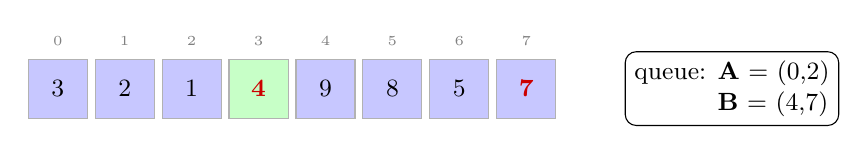
\begin{tikzpicture}
  \arr{3/cb,2/cb,1/cb,\chg{4}/cs,9/cb,8/cb,5/cb,\chg{7}/cb}
  \node[draw, rounded corners, align=left, font=\small, anchor=west] at (7.2,0)
    {queue: \textbf{A} = (0,2)\\ \phantom{queue: }\textbf{B} = (4,7)};
\end{tikzpicture}
\end{center}

%-------------------------------------------------------------------
\subsection*{Stage 2 \quad task A \texttt{(0,2)}: \texttt{hi-lo} $= 2 <$ \texttt{cutoff} $= 3$ $\Rightarrow$ \texttt{quicksort\_serial(a,0,2)}}
\noindent Loop of \texttt{quicksort\_serial(a, 0, 2)} (lines 51--55 of Listing~\ref{lst:qs}):
\begin{center}
\small
\begin{tabular}{@{}ccccclll@{}}
\toprule
iter. & \texttt{lo} & \texttt{hi} & \texttt{lo < hi} & \texttt{p} & \texttt{p-lo < hi-p} & recursive call & update \\ \midrule
1 & 0 & 2 & true & 1 & $1<1$: false & \texttt{quicksort\_serial(a, 2, 2)} & \texttt{hi = p-1 = 0} \\
2 & 0 & 0 & false & --- & --- & --- & exit loop \\
\bottomrule
\end{tabular}
\end{center}
\texttt{quicksort\_serial(a, 2, 2)} has one element: \texttt{2 < 2} is false, it returns at once.

\noindent Iteration 1 calls \texttt{partition(a, 0, 2)}, $\texttt{mid}=1$:
\begin{center}
\small
\begin{tabular}{@{}lll@{}}
\toprule
Step & Action & $a[0], a[1], a[2]$ \\ \midrule
start & --- & \cd{3} \cd{2} \cd{1} \\
$a[1]=2 < a[0]=3$ & \texttt{swap(a, 1, 0)} & \cd{\chg{2}} \cd{\chg{3}} \cd{1} \\
$a[2]=1 < a[0]=2$ & \texttt{swap(a, 2, 0)} & \cd{\chg{1}} \cd{3} \cd{\chg{2}} \\
$a[2]=2 < a[1]=3$ & \texttt{swap(a, 2, 1)} & \cd{1} \cd{\chg{2}} \cd{\chg{3}} \\
median to the end & \texttt{swap(a, 1, 2)}; pivot $=2$ & \nn{1} \nn{\chg{3}} \pv{\chg{2}} \\
$j=0,\ i=0$: $a[0]=1 < \text{pivot}=2$ & \texttt{swap(a, 0, 0)} & \sm{1} \nn{3} \pv{2} \\
$j=1,\ i=1$: $a[1]=3 \ge \text{pivot}=2$ & --- & \sm{1} \nn{3} \pv{2} \\
place pivot, $p=1$ & \texttt{swap(a, 1, 2)} & \sm{1} \pv{\chg{2}} \nn{\chg{3}} \\
\bottomrule
\end{tabular}
\end{center}
\begin{center}
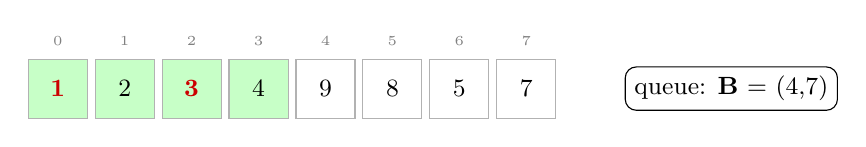
\begin{tikzpicture}
  \arr{\chg{1}/cs,2/cs,\chg{3}/cs,4/cs,9/cn,8/cn,5/cn,7/cn}
  \node[draw, rounded corners, align=left, font=\small, anchor=west] at (7.2,0)
    {queue: \textbf{B} = (4,7)};
\end{tikzpicture}
\end{center}

%-------------------------------------------------------------------
\subsection*{Stage 3 \quad task B \texttt{(4,7)}: \texttt{hi-lo} $= 3 \ge$ \texttt{cutoff} $= 3$ $\Rightarrow$ partition and create two tasks}
\texttt{partition(a,4,7)}, $\texttt{mid}=5$:
\begin{center}
\small
\begin{tabular}{@{}lll@{}}
\toprule
Step & Action & $a[4], \dots, a[7]$ \\ \midrule
start & --- & \cd{9} \cd{8} \nn{5} \cd{7} \\
$a[5]=8 < a[4]=9$ & \texttt{swap(a, 5, 4)} & \cd{\chg{8}} \cd{\chg{9}} \nn{5} \cd{7} \\
$a[7]=7 < a[4]=8$ & \texttt{swap(a, 7, 4)} & \cd{\chg{7}} \cd{9} \nn{5} \cd{\chg{8}} \\
$a[7]=8 < a[5]=9$ & \texttt{swap(a, 7, 5)} & \cd{7} \cd{\chg{8}} \nn{5} \cd{\chg{9}} \\
median to the end & \texttt{swap(a, 5, 7)}; pivot $=8$ & \nn{7} \nn{\chg{9}} \nn{5} \pv{\chg{8}} \\
$j=4,\ i=4$: $a[4]=7 < \text{pivot}=8$ & \texttt{swap(a, 4, 4)} & \sm{7} \nn{9} \nn{5} \pv{8} \\
$j=5,\ i=5$: $a[5]=9 \ge \text{pivot}=8$ & --- & \sm{7} \nn{9} \nn{5} \pv{8} \\
$j=6,\ i=5$: $a[6]=5 < \text{pivot}=8$ & \texttt{swap(a, 5, 6)} & \sm{7} \sm{\chg{5}} \nn{\chg{9}} \pv{8} \\
place pivot, $p=6$ & \texttt{swap(a, 6, 7)} & \sm{7} \sm{5} \pv{\chg{8}} \nn{\chg{9}} \\
\bottomrule
\end{tabular}
\end{center}
\begin{center}
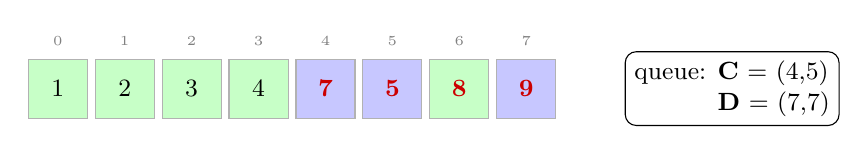
\begin{tikzpicture}
  \arr{1/cs,2/cs,3/cs,4/cs,\chg{7}/cb,\chg{5}/cb,\chg{8}/cs,\chg{9}/cb}
  \node[draw, rounded corners, align=left, font=\small, anchor=west] at (7.2,0)
    {queue: \textbf{C} = (4,5)\\ \phantom{queue: }\textbf{D} = (7,7)};
\end{tikzpicture}
\end{center}

%-------------------------------------------------------------------
\subsection*{Stage 4 \quad task C \texttt{(4,5)}: \texttt{hi-lo} $= 1 <$ \texttt{cutoff} $= 3$ $\Rightarrow$ \texttt{quicksort\_serial(a,4,5)}}
\noindent Loop of \texttt{quicksort\_serial(a, 4, 5)} (lines 51--55 of Listing~\ref{lst:qs}):
\begin{center}
\small
\begin{tabular}{@{}ccccclll@{}}
\toprule
iter. & \texttt{lo} & \texttt{hi} & \texttt{lo < hi} & \texttt{p} & \texttt{p-lo < hi-p} & recursive call & update \\ \midrule
1 & 4 & 5 & true & 4 & $0<1$: true & \texttt{quicksort\_serial(a, 4, 3)} & \texttt{lo = p+1 = 5} \\
2 & 5 & 5 & false & --- & --- & --- & exit loop \\
\bottomrule
\end{tabular}
\end{center}
\texttt{quicksort\_serial(a, 4, 3)} is an empty range: \texttt{4 < 3} is false, it returns at once.

\noindent Iteration 1 calls \texttt{partition(a, 4, 5)}, $\texttt{mid}=4$ (same cell as \texttt{lo}):
\begin{center}
\small
\begin{tabular}{@{}lll@{}}
\toprule
Step & Action & $a[4], a[5]$ \\ \midrule
start & --- & \cd{7} \cd{5} \\
$a[5]=5 < a[4]=7$ & \texttt{swap(a, 5, 4)} & \cd{\chg{5}} \cd{\chg{7}} \\
median to the end & \texttt{swap(a, 4, 5)}; pivot $=5$ & \nn{\chg{7}} \pv{\chg{5}} \\
$j=4,\ i=4$: $a[4]=7 \ge \text{pivot}=5$ & --- & \nn{7} \pv{5} \\
place pivot, $p=4$ & \texttt{swap(a, 4, 5)} & \pv{\chg{5}} \nn{\chg{7}} \\
\bottomrule
\end{tabular}
\end{center}
\begin{center}
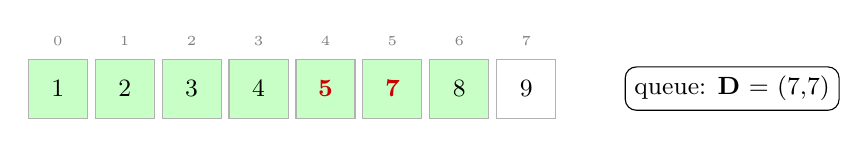
\begin{tikzpicture}
  \arr{1/cs,2/cs,3/cs,4/cs,\chg{5}/cs,\chg{7}/cs,8/cs,9/cn}
  \node[draw, rounded corners, align=left, font=\small, anchor=west] at (7.2,0)
    {queue: \textbf{D} = (7,7)};
\end{tikzpicture}
\end{center}

%-------------------------------------------------------------------
\subsection*{Stage 5 \quad task D \texttt{(7,7)}: \texttt{hi-lo} $= 0 <$ \texttt{cutoff} $= 3$ $\Rightarrow$ \texttt{quicksort\_serial(a,7,7)}}
\noindent Loop of \texttt{quicksort\_serial(a, 7, 7)} (lines 51--55 of Listing~\ref{lst:qs}):
\begin{center}
\small
\begin{tabular}{@{}ccccclll@{}}
\toprule
iter. & \texttt{lo} & \texttt{hi} & \texttt{lo < hi} & \texttt{p} & \texttt{p-lo < hi-p} & recursive call & update \\ \midrule
1 & 7 & 7 & false & --- & --- & --- & exit loop \\
\bottomrule
\end{tabular}
\end{center}
The queue is empty; T0 leaves the barrier.
\begin{center}
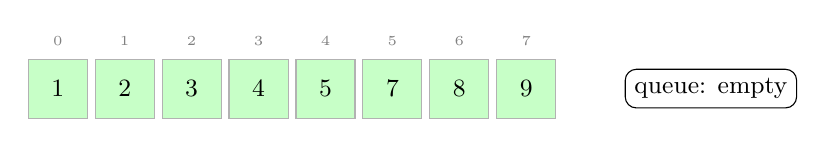
\begin{tikzpicture}
  \arr{1/cs,2/cs,3/cs,4/cs,5/cs,7/cs,8/cs,9/cs}
  \node[draw, rounded corners, align=left, font=\small, anchor=west] at (7.2,0)
    {queue: empty};
\end{tikzpicture}
\end{center}

%-------------------------------------------------------------------
\section{The code}\label{sec:code}
\lstinputlisting[caption={\textbf{\origtexttt{quicksort\_tasks.c}} -- parallel quicksort with tasks.}, label={lst:qs}]{quicksort_tasks.c}

\begin{lstlisting}[style=sh]
gcc -Wall -O2 -fopenmp -o quicksort_tasks quicksort_tasks.c
OMP_NUM_THREADS=2 ./quicksort_tasks 20000000 10000
\end{lstlisting}
Output on a 2-core machine (your times will differ):
\begin{lstlisting}[style=sh]
n = 20000000, cutoff = 10000, threads = 2
serial : 2.534 s
tasks  : 1.289 s   speed-up 1.97   sorted: yes
work per thread (elements sorted in serial pieces):
  thread  0:    9305664 elements in   1577 pieces ( 46.5%)
  thread  1:   10690906 elements in   1854 pieces ( 53.5%)
\end{lstlisting}
The percentages add up to slightly less than 100\% because the pivots are placed by the
partitions, not by the serial pieces.

\begin{keyidea}
\begin{itemize}
  \item Tasks fit work whose shape appears while it runs: trees, recursion, irregular sizes.
  \item Load balance comes for free: a thread that finishes a small piece takes the next
        task; nobody decides the distribution in advance.
  \item \texttt{taskwait} only where results are needed; the barrier of the region collects
        the rest.
  \item Tasks that write disjoint parts of a shared array need no synchronization.
\end{itemize}
\end{keyidea}

\section{Experiments}

\subsection*{Experiment 1: work distribution and speed-up}
\begin{experiment}
\textbf{Question:} how well does the irregular work spread over the threads, and what
limits the speed-up?
\begin{enumerate}
  \item Run with an increasing number of threads:
\begin{lstlisting}[style=sh]
for t in 1 2 4 $(nproc); do
    OMP_NUM_THREADS=$t ./quicksort_tasks 20000000 10000
done
\end{lstlisting}
  \item For each run, note the speed-up and the smallest and largest share of work in the
        per-thread table.
\end{enumerate}
\textbf{What to observe and answer.}
\begin{enumerate}
  \item The threads sort different numbers of pieces and elements, yet the speed-up stays
        close to the number of threads. Why does unequal \emph{work} not mean idle threads?
  \item Run the same command twice. Does the distribution of work change? Why?
  \item The first partition runs on one thread, before any task exists. Why does it limit
        the speed-up on machines with many cores?
\end{enumerate}
\end{experiment}

\paragraph{Answers (read after trying).}

\noindent(1)~Every thread keeps taking tasks until none are left, so all threads stay busy
until the end. A thread that happened to draw small pieces simply takes more of them.
Unequal shares only show that the pieces had different sizes, not that anyone waited. (With
8 threads on 2 million elements, the shares ranged from 8\% to 16.5\%.)

\noindent(2)~Yes. Which thread takes which task depends on timing, which changes every run.
The \emph{result} does not change, because each piece is sorted correctly by whoever takes
it.

\noindent(3)~Before the first partition finishes there is only one piece and only one thread
can work; the second level offers only two pieces, and so on. On the test machine the first
partition alone took 0.042\,s of the 2.43\,s serial sort, and the chain of partitions down
to the largest piece adds more. This serial part (Amdahl's law) caps the speed-up at roughly
$2.43/0.12\approx20$ on this input, no matter how many cores. Parallelizing the partition
itself removes this limit, at the cost of a more complex algorithm.

\subsection*{Experiment 2: choosing the cutoff}
\begin{experiment}
\textbf{Question:} which \texttt{cutoff} gives the best time, and why?
\begin{enumerate}
  \item Time \texttt{quicksort\_tasks} for cutoffs from $10^2$ to $n$ with all your cores
        (Listing~\ref{lst:run}):
\begin{lstlisting}[style=sh]
sh run_cutoff.sh 20000000 $(nproc)
\end{lstlisting}
        It writes \texttt{cutoff.dat}: plain text, one line per cutoff, columns separated by
        spaces (1: cutoff, 2: serial time, 3: tasks time, 4: speed-up); lines starting with
        \texttt{\#} are comments. Any plotter can read it (gnuplot, Python
        \texttt{numpy.loadtxt}, a spreadsheet).
  \item Plot it with gnuplot (Listing~\ref{lst:plot}), which writes \texttt{cutoff.png}:
\begin{lstlisting}[style=sh]
gnuplot plot_cutoff.gp
\end{lstlisting}
\end{enumerate}
\textbf{What to observe and answer.}
\begin{enumerate}
  \item What happens to the speed-up when the cutoff is close to $n$? And at
        $\texttt{cutoff} = n$?
  \item Does a very small cutoff (100) hurt on your machine? Why could it?
  \item Which range of cutoffs is good, and how would you choose one for a different $n$ or
        number of threads?
\end{enumerate}
\end{experiment}

\lstinputlisting[language=sh, caption={\textbf{\origtexttt{run\_cutoff.sh}} -- time the sort for several cutoffs and write \origtexttt{cutoff.dat}.}, label={lst:run}]{run_cutoff.sh}

\lstinputlisting[language={}, caption={\textbf{\origtexttt{plot\_cutoff.gp}} -- gnuplot script: time and speed-up against the cutoff.}, label={lst:plot}]{plot_cutoff.gp}

\paragraph{Answers (read after trying).} Figure~\ref{fig:cutoff} shows two runs on the
author's laptop with $n = 2\cdot10^7$: 2 threads and 8 threads.
\begin{figure}[htbp]
\centering
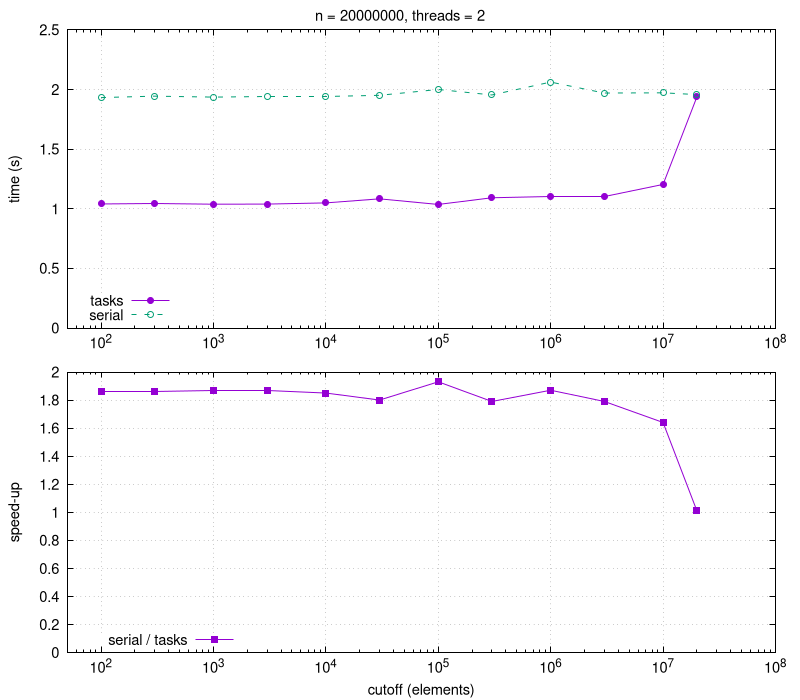
\includegraphics[width=0.49\linewidth]{cutoff_2.png}\hfill
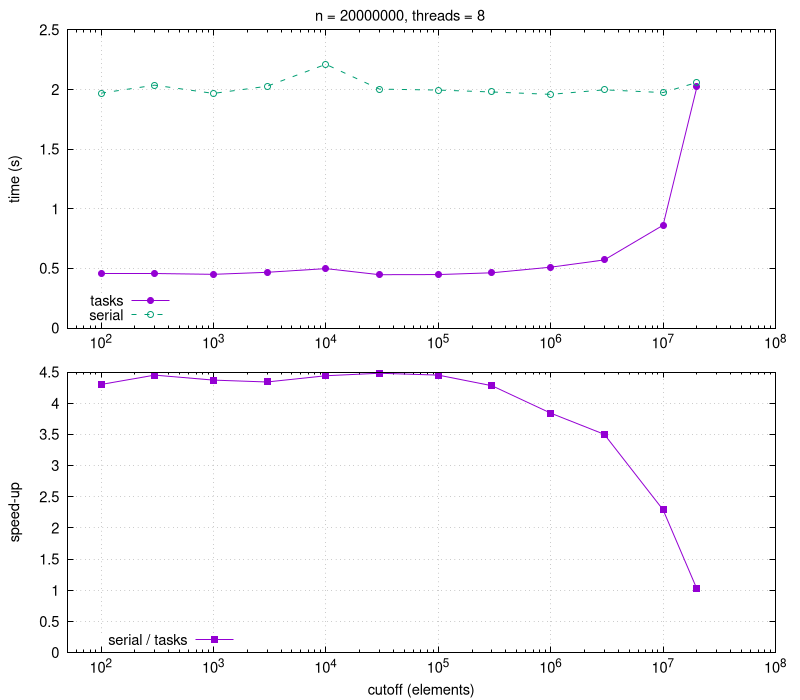
\includegraphics[width=0.49\linewidth]{cutoff_8.png}
\caption{\texttt{cutoff.png} for $n = 2\cdot10^7$: 2 threads (left), 8 threads (right).}\label{fig:cutoff}
\end{figure}

\noindent(1)~With a large cutoff only a few pieces become tasks: about $n/\texttt{cutoff}$
serial pieces, of unequal size, so some thread finishes late. With 2 threads this only shows
at $\texttt{cutoff}=10^7$ (2 pieces, speed-up 1.6). With 8 threads the drop starts earlier,
because 8 threads need more pieces: 3.8 at $10^6$, 2.3 at $10^7$. At $\texttt{cutoff}=n$ the
very first call is already below the cutoff and sorts everything serially: no task is
created, and the speed-up is 1.

\noindent(2)~Each task costs some time to create and schedule (about a microsecond, Lesson~12).
A cutoff of 100 creates hundreds of thousands of tasks. With 2 threads this costs nothing
visible (1.86, against the best 1.93); with 8 threads it costs a little (4.3, against the
best 4.5). The overhead grows with the number of tasks and threads.

\noindent(3)~The flat part of the curve: from $10^2$ to about $3\cdot10^6$ with 2 threads, but
only to about $10^5$ with 8 threads: more threads move the right edge to the left. A safe
choice keeps both conditions true: many more pieces than threads ($n/\texttt{cutoff} \gg$
threads, e.g.\ at least 100 per thread) and pieces large enough to hide the task overhead
(thousands of elements). For $n=2\cdot10^7$ and 8 threads, a cutoff around $10^4$ satisfies
both.

\paragraph{Next lesson.} \texttt{taskloop} and task dependencies (\texttt{depend}).

\begin{thebibliography}{9}
\bibitem{vdp} R.~van der Pas, E.~Stotzer, and C.~Terboven. \emph{Using OpenMP --- The Next
  Step: Affinity, Accelerators, Tasking, and SIMD}. MIT Press, Cambridge, MA, 2017.
\end{thebibliography}
\end{document}
